\documentclass[tikz]{standalone}
\usetikzlibrary{automata,positioning}
\begin{document}
  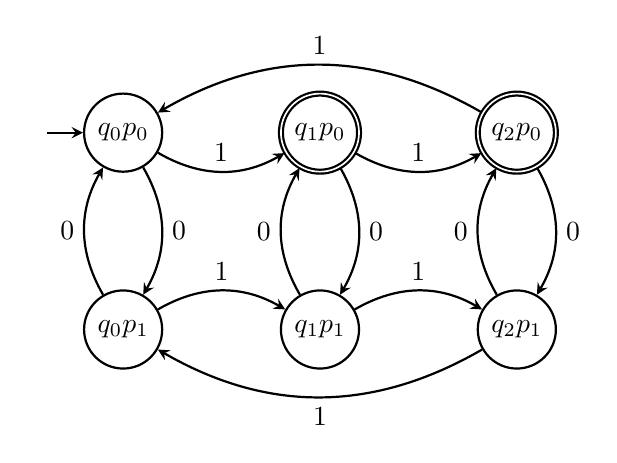
\begin{tikzpicture}[>=stealth,node distance=25mm,on grid,auto, thick, initial text=]
    \node[state,initial] (r00) {$q_0p_0$};
    \node[state,accepting] (r10) [right=of r00] {$q_1p_0$};
    \node[state,accepting] (r20) [right=of r10] {$q_2p_0$};
    \node[state] (r01) [below=of r00] {$q_0p_1$};
    \node[state] (r11) [right=of r01] {$q_1p_1$};
    \node[state] (r21) [right=of r11] {$q_2p_1$};
    
    \path[->]
    (r00) edge [bend right] node {1} (r10)
    (r10) edge [bend right] node {1} (r20)
    (r01) edge [bend left] node {1} (r11)
    (r11) edge [bend left] node {1} (r21)
    (r20) edge [bend right] node [above] {1} (r00)
    (r21) edge [bend left] node {1} (r01)
    (r00) edge [bend left] node {0} (r01)
    (r01) edge [bend left] node {0} (r00)
    (r10) edge [bend left] node {0} (r11)
    (r11) edge [bend left] node {0} (r10)
    (r21) edge [bend left] node {0} (r20)
    (r20) edge [bend left] node {0} (r21);    
  \end{tikzpicture}

\end{document}